\begin{appendix}
\chapter{Software \& Technologies}
In this appendix we will present the details of the software and the technologies used for achieving this
work.

\begin{itemize}
\item \textbf{Software environment:}
\begin{itemize}
\item \textbf{Microsoft Visual Studio:}\\
Microsoft Visual Studio is an integrated development environment (IDE) developed by Microsoft. It is
used for developing web sites, web services and in our case, web applications.
This software includes code editor, components for code completion, debugger and other features
offering a multitude of options for developers. This IDE supports different programming languages
such as C\#, HTML, JavaScript and many others.
\item \textbf{Microsoft SQL Server:}\\
Microsoft SQL Server is a relational database management system from Microsoft. It offers a set of programming extensions that add several features to standard SQL including row processing,
error handling and transaction control.
\item \textbf{Spyder:}\\
Spyder is an open source cross-platform integrated development environment (IDE) for scientific programming in the Python language. Spyder integrates NumPy, SciPy, Matplotlib and IPython, as well as other open source software. Spyder is extensible with plugins, includes support for interactive tools for data inspection and embeds Python-specific code quality assurance and introspection instruments. It is available cross-platform through Anaconda, on Windows with WinPython and Python(x,y).
\item \textbf{Anaconda:}\\
Anaconda is a freemium open source distribution of the Python and R programming languages for large-scale data processing, predictive analytics, and scientific computing, that aims to simplify package management and deployment. Package versions are managed by the package management system conda.
\item \textbf{Microsoft Project:}\\
Microsoft Project is a project management software developed by Microsoft. It helps plan, organize
and manage estimation, planning and scheduling. We used this software in order to keep the work
organized and respect the time lines for the project's different steps.
\newpage
\end{itemize}
\item \textbf{Technologies:}
\begin{itemize}
\item \textbf{C\# Programming Language:}\\
C\# is an object oriented programming language from Microsoft. It enables
developers to build secure and robust applications. It also permits to develop applications that run on the .Net framework.
\item \textbf{ASP.NET Framework:}\\
Asp.net is a free web framework used for developing and building
web applications using different languages such as HTML, CSS, JavaScript and many others. This web framework offers three different frameworks for creating web applications: ASP.NET Web Pages, ASP.NET Web Forms, ASP.NET MVC. All of the three frameworks mentioned above offers the
same facilities that are part of the core ASP.NET framework.
\item \textbf{DevExpress:}\\
DevExpress is a custom third party provider of .NET controls. They customize the .NET controls by making it more attractive and more flexible than inbuilt .NET controls.
\item \textbf{Python Programming Language:}\\
Python is a powerful high-level, object-oriented programming language. Python is an interpreted language, it has a design philosophy which emphasizes code readability through whitespace indentation, and a syntax which allows programmers to express concepts in few lines code. 
\item \textbf{Apache Spark Framework:}\\
Apache Spark is a fast and general engine for large-scale data processing. Spark powers a stack of libraries including SQL and DataFrames, MLlib for machine learning, GraphX, and spark Streaming. Spark extends its predecessors with in-memory processing. Its Resilient Distributed Dataset (RDD) abstraction enables developers to materialize any point in a processing pipeline into memory across the cluster, meaning that future steps that want to deal with the same data set need not recompute it or reload it from disk. Sparks runs on Hadoop, Mesos, standalone, or in the cloud.
\item \textbf{Hadoop Distributed File System (HDFS):}\\
HDFS is a distributed file system that provides high-performance access to data across Hadoop clusters. Like other Hadoop-related technologies, HDFS has become a key tool for managing pools of big data and supporting big data analytics applications.
\item \textbf{Bootstrap Framework:}\\
Bootstrap is an open-source Javascript framework developed by the team at Twitter. It is a combination of HTML, CSS, and Javascript code designed to help build user interface components.
\end{itemize}
\end{itemize}





\chapter{Achievements}
\label{achievement}
In this appendix we will show the different steps that should be followed to process an algorithm on a data.

~\\
~\\
~\\
~\\
~\\
~\\
~\\
~\\
\begin{itemize}
\item \textbf{Step 1:} Register\\

\begin{figure}[!ht]
\begin{center}
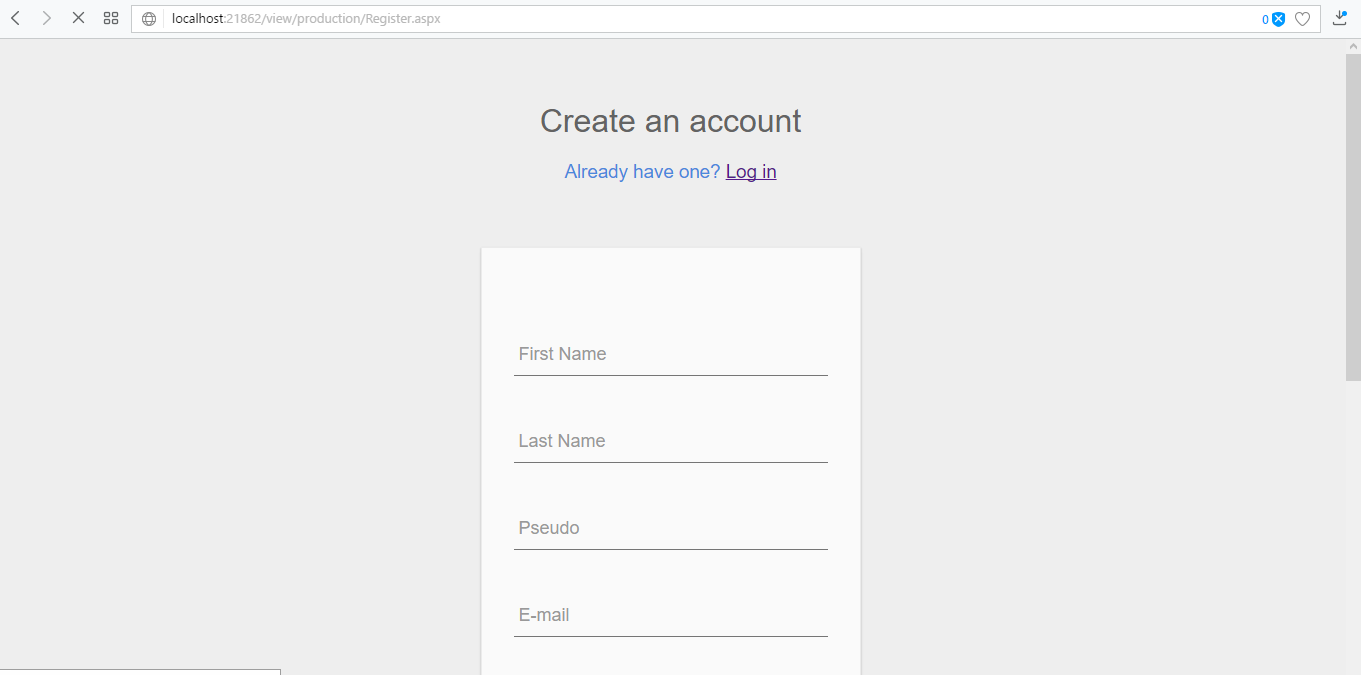
\includegraphics[width=17cm,height=10cm]{chapter5/register.png}
\end{center}
\caption{Register Page Capture}
\label{register}
\end{figure} 

\item \textbf{Step 2:} Login\\

\begin{figure}[!ht]
\begin{center}
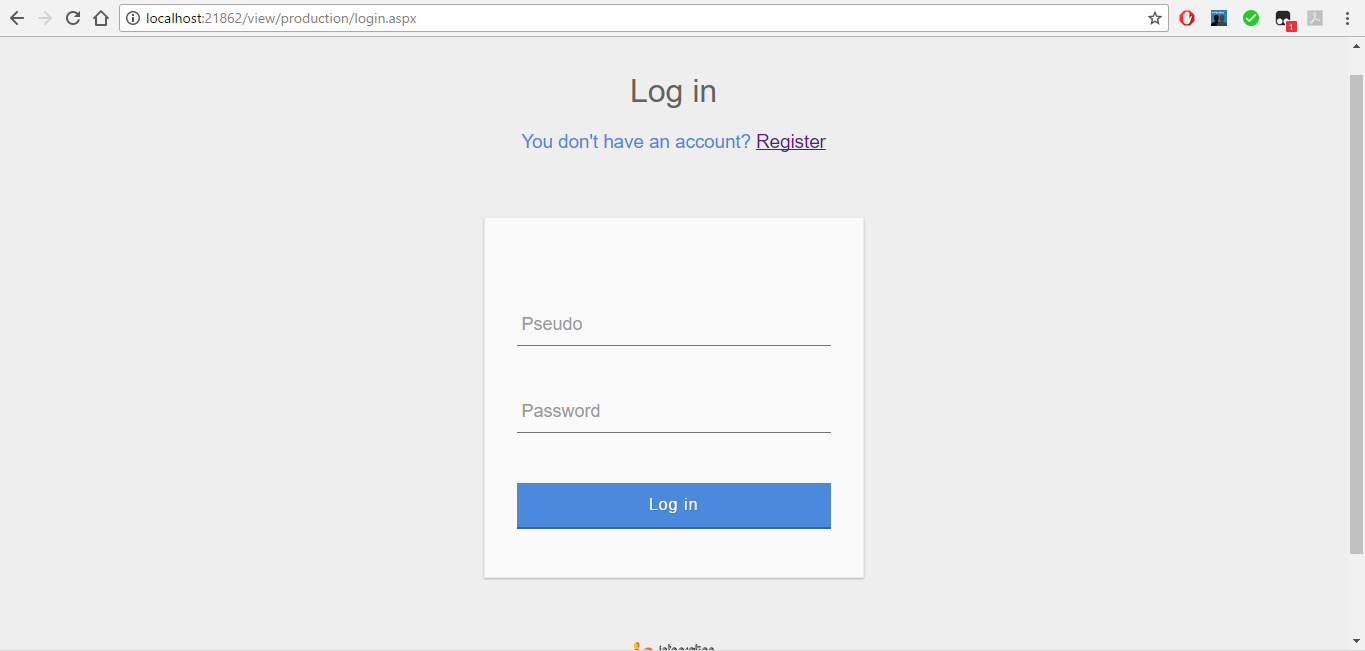
\includegraphics[width=17cm,height=10cm]{chapter5/login.png}
\end{center}
\caption{Login Page Capture}
\label{login}
\end{figure} 

\item \textbf{Step 3:} Load Data\\

\begin{figure}[!ht]
\begin{center}
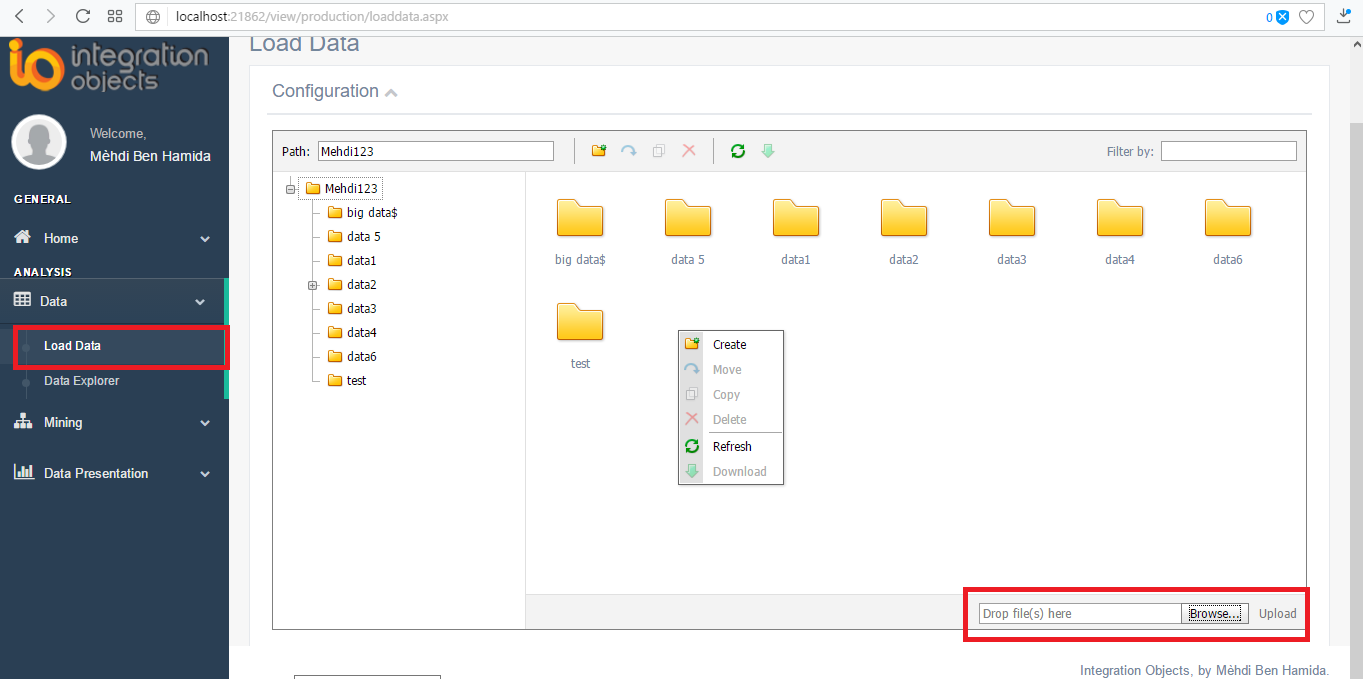
\includegraphics[width=17cm,height=10cm]{chapter5/load.png}
\end{center}
\caption{Load Page Capture}
\label{l}
\end{figure} 


\item \textbf{Step 4:} Select an algorithm\\

\begin{figure}[!ht]
\begin{center}
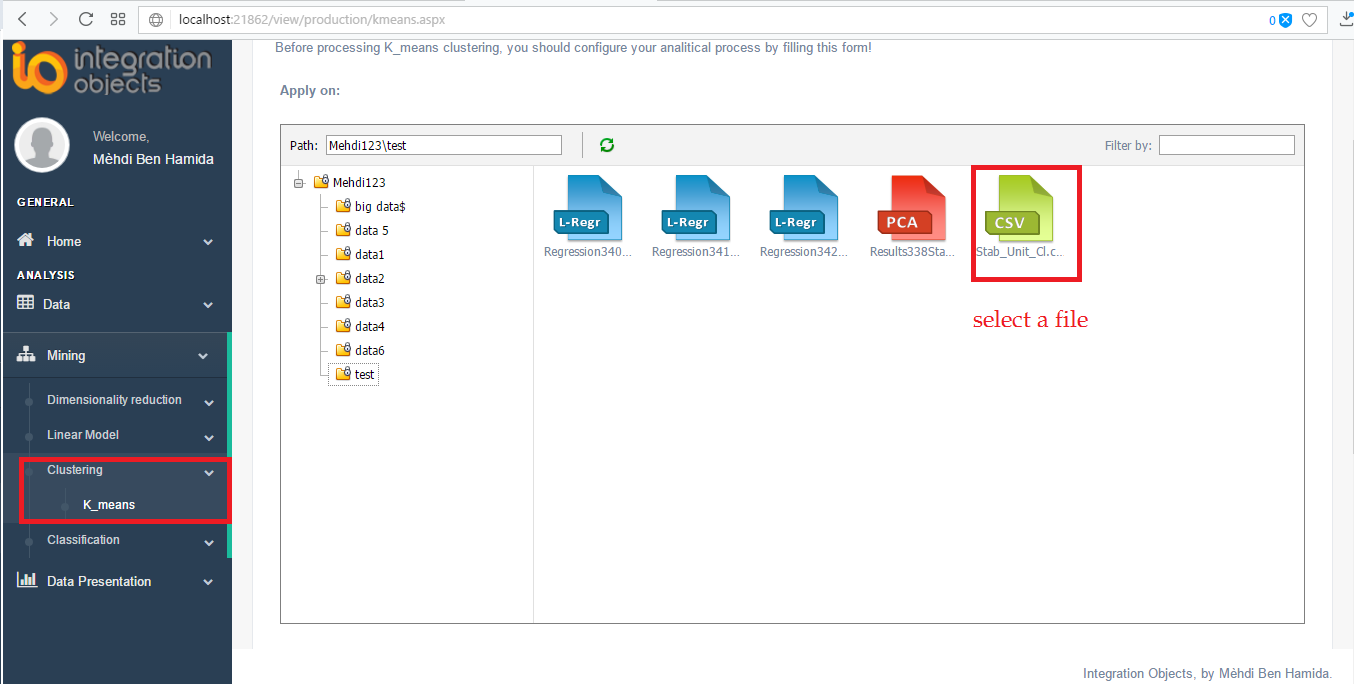
\includegraphics[width=17cm,height=10cm]{chapter5/k1.png}
\end{center}
\caption{Select Algorithm Page Capture}
\label{s}
\end{figure} 

\item \textbf{Step 5:} Set algorithm parameters\\

\begin{figure}[!ht]
\begin{center}
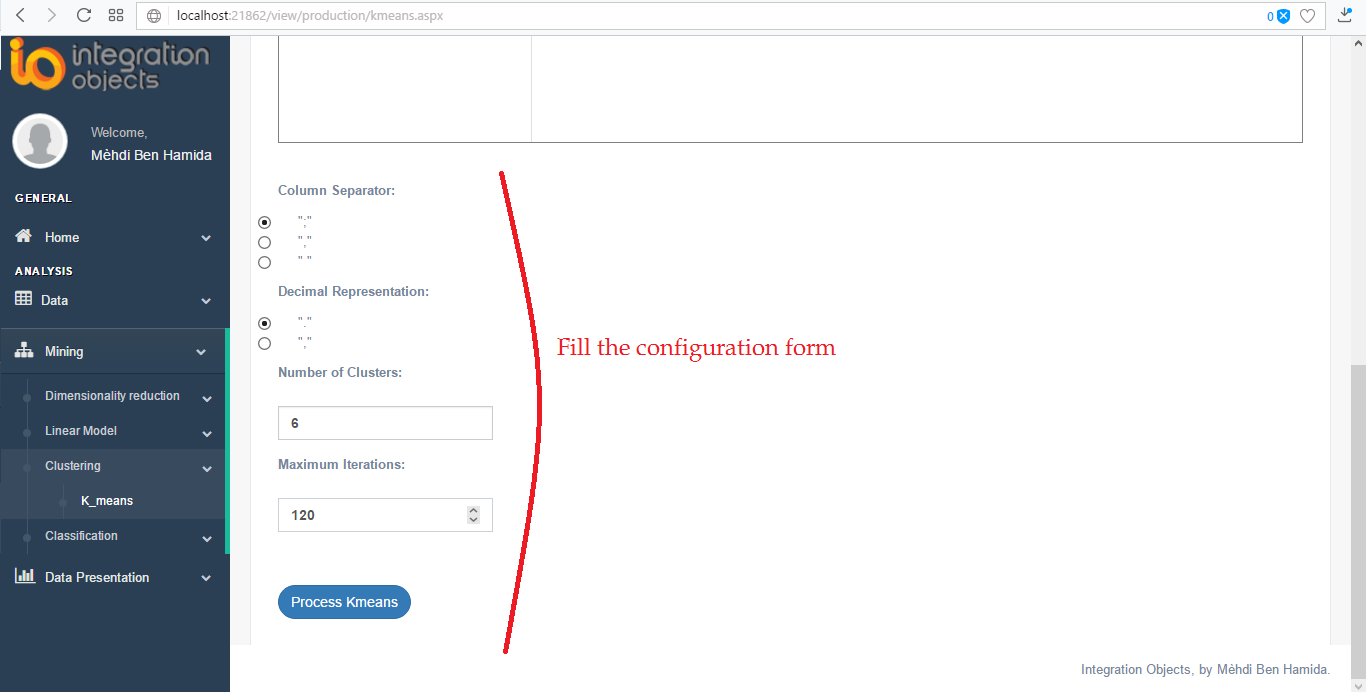
\includegraphics[width=17cm,height=10cm]{chapter5/k2.png}
\end{center}
\caption{Set Algorithm Parameters Page Capture}
\label{s2}
\end{figure} 

\item \textbf{Step 6:} Set chart parameters\\

\begin{figure}[!ht]
\begin{center}
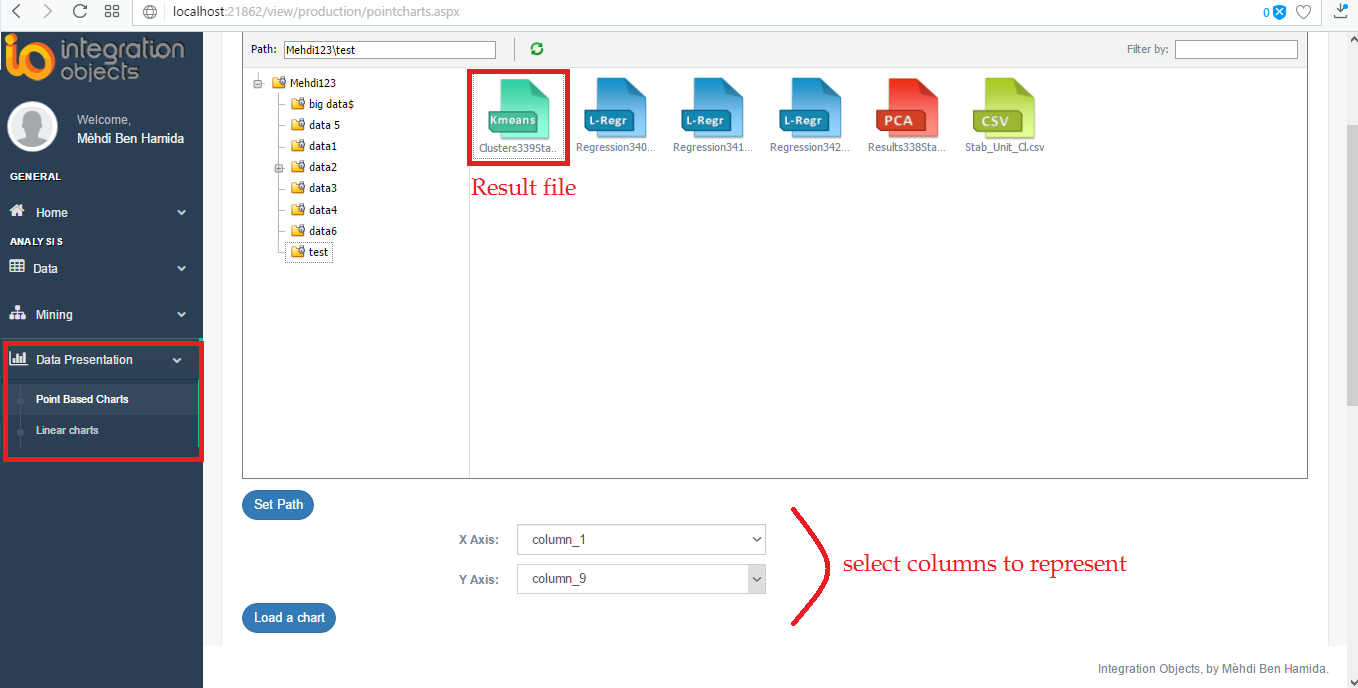
\includegraphics[width=17cm,height=10cm]{chapter5/kc1.png}
\end{center}
\caption{Set chart Parameters Page Capture}
\label{s3}
\end{figure} 


\item \textbf{Step 7:} Load chart\\


\begin{figure}[!ht]
\begin{center}
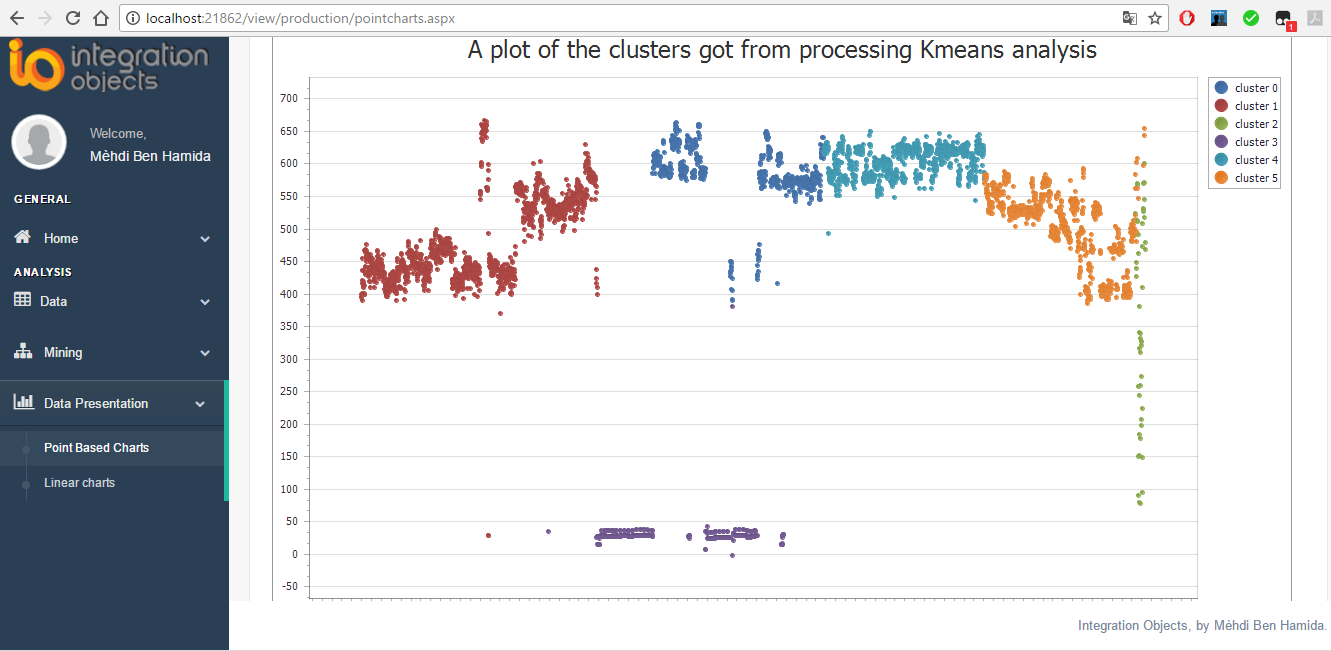
\includegraphics[width=17cm,height=10cm]{chapter5/kmeans.png}
\end{center}
\caption{Result Chart Capture}
\label{k}
\end{figure} 


\end{itemize}





\chapter{Principal Component Analysis}
\label{appendixpca}
The main problem of principal component analysis is represented by the equation represented in section \ref{sectionpca}:

\begin{equation*}
PX = (Px_{1} Px_{2} \ldots Px_{n})
=
\begin{pmatrix}
    p_{1}x_{1} & p_{1}x_{2}  & \dots  & p_{1}x_{n} \\
    p_{2}x_{1} & p_{2}x_{2}  & \dots  & p_{2}x_{n} \\
    \vdots & \vdots  & \ddots & \vdots \\
    p_{m}x_{1} & p_{m}x_{2}  & \dots  & p_{m}x_{n}
\end{pmatrix}
=
Y
\end{equation*}

Principal Components Analysis defines independence by considering the variance of the data in the original basis. It seeks to de-correlate the original data by finding the directions in which variance is maximised and the us these directions to define the new basis. Recall the definition for the variance of a random variable, $Z$ with mean, $\mu$.\\
\begin{equation*}
\sigma_{Z}^{2}=E[(Z-\mu )^{2}]
\end{equation*}

Suppose we have a vector of $n$ discrete measurement with mean $\mu_{r}$, if we subtract the mean from each of the measurement, then we obtain a translated set of measurement $r=(r_{1},r_{2},\ldots, r_{n},)$, that has zero mean. Thus, the variance of these measurement is given by the relation:\\
\begin{equation*}
\sigma_{r}^{2}=\frac{1}{n}rr^{T}
\end{equation*}

Suppose that we have a second vector of n measurement, $s = (s_{1}, s_{2}, \ldots ,s_{n})$, with zero mean, then we generalize this idea to obtain the covariance of $r$ and $s$. Covariance can be thought of as a measure of how much two variable change together. Variance is thus a special case of covariance, when the two variables are identical. It is in fact correct to divide through by a factor of $n-1$ rather than $n$.\\
\begin{equation*}
\sigma_{rs}^{2}=\dfrac{1}{n-1}rs^{T}
\end{equation*}

We can now generalize this idea to considering our $m \times n$ data matrix, $X$. Recall that m was the number of variables, and n the number of sample. We can therefore think of this matrix, $X$ in terms of $m$ row vectors, each of length n.\\
\begin{equation*}
X
=
\begin{pmatrix}
x_{1,1}&x_{1,2}&\cdots&x_{1,n}\\
x_{2,1}&x_{2,2}&\cdots&x_{2,n}\\
\vdots&\vdots&\ddots&\vdots\\
x_{m,1}&x_{m,1}&\cdots&x_{m,n}
\end{pmatrix} 
=
\begin{pmatrix}
X1\\
X2\\
\vdots\\
X_{m}
\end{pmatrix}
\in \mathbb{R}^{m\times n},\quad x_{i}^{T} \in \mathbb{R}^{n}
\end{equation*}

Since we have a row vector for each variable, each of these vectors contains all the samples for one particular variable. So for example, $x_{i}$ is a vector of the $n$ samples for the $i^{th}$ variable. It therefore makes sense to consider the following matrix product.\\
\begin{equation*}
C_{X}=\dfrac{1}{n-1}XX^{T}=\dfrac{1}{n-1}\begin{pmatrix}
X_{1}X_{1}^{T}&X_{1}X_{2}^{T}&\cdots &X_{1}X_{m}^{T}\\
X_{2}X_{1}^{T}&X_{2}X_{2}^{T}&\cdots &X_{2}X_{m}^{T}\\
\vdots &\vdots &\ddots &\vdots \\
X_{m}X_{1}^{T}&X_{m}X_{2}^{T}&\cdots &X_{m}X_{m}^{T}
\end{pmatrix}
\in \mathbb{R}^{m\times m}
\end{equation*}

If we look closely at the entries of this matrix, we see that we have computed all the possible covariance pairs between the $m$ variables. Indeed, on the diagonal entries, we have the variances and on the off-diagonal entries, we have the covariances. This matrix is therefore known as the Covariance Matrix.\\

Now let us return to the original problem, that of linearly transforming the original data matrix using the relation $Y=PX$, for some matrix, $P$. We need to decide upon some features that we would like the transformed matrix, $Y$ to exhibit and somehow relate this to the feature of the corresponding covarience matrix $C_{Y}$.\\

Covariance can be considered to be a mesure of how well correlated two variables are. The PCA method makes the fundamental assumption that the variables in the transformed matrix $C_{Y}$, should be as close to zero as possible (covariance matrices are always positive definite or positive semi-definite). Conversely, large variance values interest us, since they correspond to interesting dynamics in the system (small variances may well be noises). we therefore have the following requirements for constructing the covariance matrix, $C_{Y}$
\begin{itemize}
\item Maximise the signal, measured by variance (maximise the diagonal entries)
\item Minimise the covariance between variables (minimise the off-diagonal entries)\\
\end{itemize}

We thus come to the conclusion that since the minimum possible covariance is zero, we are seeking a diagonal matrix, $C_Y$. If we can choose the transformation matrix, $P$ in such a way that $C_Y$ is diagonal, then we will have achieved our objective.\\

We now make the assumption that the vectors in the new basis, $p_{1}, p_{2},\ldots , p_{m}$ are orthogonal (in fact, we additionally assume that they are orthonormal). Far from being restrictive, this assumption enables us to proceed by using the tools of linear algebra to find a solution to the problem. Consider the formula for the covariance matrix, $C_Y$ and our interpretation of $Y$ in terms of $X$ and $P$.\\
\begin{equation*}
\begin{multlined}
C_{Y} = \dfrac{1}{n-1} YY^{T} = \dfrac{1}{n-1} (PX)(PX)^T = \dfrac{1}{n-1} (PX)(X^{T}P^{T}) = \frac{1}{n-1} P(XX^{T})P^{T} \\
\quad \textrm{i.e} \quad C_{Y} = \dfrac{1}{n-1} PSP^{T} \quad \textrm{where} \quad  S = XX^{T}
\end{multlined}
\end{equation*}

Note that $S$ is an $ m \times n$ symmetric matrix, since $(XX^{T})^T = (X^T)^T(X)^{T}=XX^{T}$. We now invoke the well known theorem for linear algebra that every square symmetric matrix is orthogonally  (orthonormally) diagonalisable. That is, we can write:\\

\begin{equation*}
S=EDE^{T}
\end{equation*} 

Where E is an $m \times m$ orthonormal matrix whose columns are the orthonormal eigenvectors of $S$, and $D$ is the number of orthonormal eigenvectors that it has. if $B$ turns out to be rank-deficient so that $r$ is less than the size, $m$, of the matrix, then we simply need to generate $m-r$ orthonormal vectors to fill the remaining columns of $S$.\\
 
It is at this point that we make a choice for the transformation matrix, $P$. By choosing the rows of $P$ to be the eigenvectors of $S$, we ensure that $P=E^{T}$ and vice versa. Thus, substituting this into our derived expression for the covariance matrix, $C_Y$ gives:\\
\begin{equation*}
C_{Y} = \dfrac{1}{n-1}PSP^{T}=\dfrac{1}{n-1}E^{T}(EDE^{T})E
\end{equation*}

Now, since $E$ is an orthonormal matrix, we have $E^{T}E=I$ is the $m \times m$ identity matrix. Hence, for this special choice of $P$, we have:\\
\begin{equation*}
C_{Y}=\dfrac{1}{n-1}D
\end{equation*} 

A last point to note is that with this method, we automatically gain information about the relative importance of each principal component from the variances. The largest variance corresponds to the first principal component, the second largest to the second principal component, and so on. This therefore gives us a method for organising the data in the diagonalisation stage. Once we have obtained the eigenvalues and eigenvectors of $S = XX^{T}$, we sort the eigenvalues in descending order and place them in this order on the diagonal of $D$. We then construct the orthonormal matrix, $E$ by placing the associated eigenvectors in the same order to form the columns of $E$ (i.e. place the eigenvector that corresponds to the largest eigenvalue in the first column, the eigenvector corresponding to the second largest eigenvalue in the second column etc.).\\

We have therefore achieved our objective of diagonalising the covariance matrix of the
transformed data. The principal components (the rows of $P$) are the eigenvectors of the covariance matrix, $XX^{T}$, and the rows are in order of importance, telling us how principal each principal component is.

\end{appendix}